% ! TEX root = ./introductory_thoughts.tex
\tikzset{every picture/.style={line width=0.75pt}} %set default line width to 0.75pt        

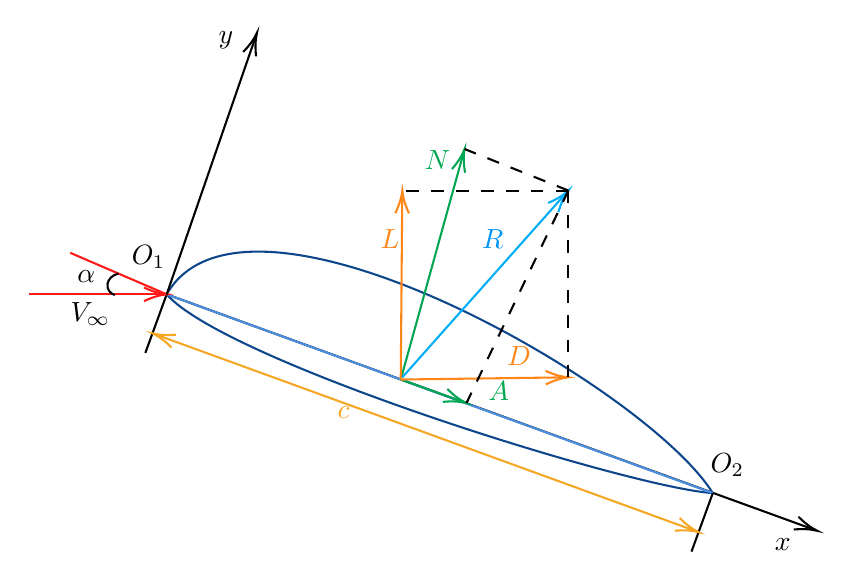
\begin{tikzpicture}[x=0.75pt,y=0.75pt,yscale=-1,xscale=1]
	%uncomment if require: \path (0,353); %set diagram left start at 0, and has height of 353

	%Straight Lines [id:da1842109967268275] 
	\draw    (186.47,136.04) -- (498.12,249.32) ;
	\draw [shift={(500,250)}, rotate = 199.97] [color={rgb, 255:red, 0; green, 0; blue, 0 }  ][line width=0.75]    (10.93,-3.29) .. controls (6.95,-1.4) and (3.31,-0.3) .. (0,0) .. controls (3.31,0.3) and (6.95,1.4) .. (10.93,3.29)   ;
	%Curve Lines [id:da035648358588663775] 
	\draw [color={rgb, 255:red, 14; green, 70; blue, 139 }  ,draw opacity=1 ]   (186.47,136.04) .. controls (224.32,69.81) and (417.44,180.11) .. (449.59,231.81) ;
	%Curve Lines [id:da2965896641352135] 
	\draw [color={rgb, 255:red, 14; green, 70; blue, 139 }  ,draw opacity=1 ]   (186.47,136.04) .. controls (214.79,168.5) and (409.77,229.25) .. (449.59,231.81) ;
	%Straight Lines [id:da05743983968805111] 
	\draw [color={rgb, 255:red, 74; green, 144; blue, 226 }  ,draw opacity=1 ]   (186.47,136.04) -- (449.59,231.81) ;
	%Straight Lines [id:da10439448052891231] 
	\draw    (449.59,231.81) -- (439.33,260) ;
	%Straight Lines [id:da788041337249308] 
	\draw    (186.47,136.04) -- (176.21,164.23) ;
	%Straight Lines [id:da7611175858700716] 
	\draw [color={rgb, 255:red, 245; green, 166; blue, 35 }  ,draw opacity=1 ]   (292.4,195.88) -- (440.87,249.92) ;
	\draw [shift={(442.75,250.6)}, rotate = 200] [color={rgb, 255:red, 245; green, 166; blue, 35 }  ,draw opacity=1 ][line width=0.75]    (10.93,-3.29) .. controls (6.95,-1.4) and (3.31,-0.3) .. (0,0) .. controls (3.31,0.3) and (6.95,1.4) .. (10.93,3.29)   ;
	%Straight Lines [id:da4556885360753773] 
	\draw [color={rgb, 255:red, 245; green, 166; blue, 35 }  ,draw opacity=1 ][fill={rgb, 255:red, 245; green, 166; blue, 35 }  ,fill opacity=1 ]   (292.4,195.88) -- (181.51,155.52) ;
	\draw [shift={(179.63,154.84)}, rotate = 20] [color={rgb, 255:red, 245; green, 166; blue, 35 }  ,draw opacity=1 ][line width=0.75]    (10.93,-3.29) .. controls (6.95,-1.4) and (3.31,-0.3) .. (0,0) .. controls (3.31,0.3) and (6.95,1.4) .. (10.93,3.29)   ;
	%Straight Lines [id:da3164870624705869] 
	\draw [color={rgb, 255:red, 0; green, 166; blue, 82 }  ,draw opacity=1 ]   (299.24,177.09) -- (329.47,67.96) ;
	\draw [shift={(330,66.04)}, rotate = 105.48] [color={rgb, 255:red, 0; green, 166; blue, 82 }  ,draw opacity=1 ][line width=0.75]    (10.93,-3.29) .. controls (6.95,-1.4) and (3.31,-0.3) .. (0,0) .. controls (3.31,0.3) and (6.95,1.4) .. (10.93,3.29)   ;
	%Straight Lines [id:da47805468728724976] 
	\draw [color={rgb, 255:red, 0; green, 166; blue, 82 }  ,draw opacity=1 ]   (299.24,177.09) -- (329.03,187.78) ;
	\draw [shift={(330.91,188.45)}, rotate = 199.74] [color={rgb, 255:red, 0; green, 166; blue, 82 }  ,draw opacity=1 ][line width=0.75]    (10.93,-3.29) .. controls (6.95,-1.4) and (3.31,-0.3) .. (0,0) .. controls (3.31,0.3) and (6.95,1.4) .. (10.93,3.29)   ;
	%Straight Lines [id:da9044725657133146] 
	\draw [color={rgb, 255:red, 255; green, 25; blue, 25 }  ,draw opacity=1 ]   (120,136.04) -- (184.47,136.04) ;
	\draw [shift={(186.47,136.04)}, rotate = 180.01] [color={rgb, 255:red, 255; green, 25; blue, 25 }  ,draw opacity=1 ][line width=0.75]    (10.93,-3.29) .. controls (6.95,-1.4) and (3.31,-0.3) .. (0,0) .. controls (3.31,0.3) and (6.95,1.4) .. (10.93,3.29)   ;
	%Straight Lines [id:da007233215583360764] 
	\draw [color={rgb, 255:red, 255; green, 134; blue, 24 }  ,draw opacity=1 ]   (299.24,177.09) -- (299.98,88.04) ;
	\draw [shift={(300,86.04)}, rotate = 90.48] [color={rgb, 255:red, 255; green, 134; blue, 24 }  ,draw opacity=1 ][line width=0.75]    (10.93,-3.29) .. controls (6.95,-1.4) and (3.31,-0.3) .. (0,0) .. controls (3.31,0.3) and (6.95,1.4) .. (10.93,3.29)   ;
	%Straight Lines [id:da3618051683565324] 
	\draw [color={rgb, 255:red, 255; green, 134; blue, 24 }  ,draw opacity=1 ]   (299.24,177.09) -- (378,176.06) ;
	\draw [shift={(380,176.04)}, rotate = 179.26] [color={rgb, 255:red, 255; green, 134; blue, 24 }  ,draw opacity=1 ][line width=0.75]    (10.93,-3.29) .. controls (6.95,-1.4) and (3.31,-0.3) .. (0,0) .. controls (3.31,0.3) and (6.95,1.4) .. (10.93,3.29)   ;
	%Straight Lines [id:da04699365108287412] 
	\draw [color={rgb, 255:red, 0; green, 174; blue, 247 }  ,draw opacity=1 ]   (300,176.04) -- (378.67,87.53) ;
	\draw [shift={(380,86.04)}, rotate = 131.63] [color={rgb, 255:red, 0; green, 174; blue, 247 }  ,draw opacity=1 ][line width=0.75]    (10.93,-3.29) .. controls (6.95,-1.4) and (3.31,-0.3) .. (0,0) .. controls (3.31,0.3) and (6.95,1.4) .. (10.93,3.29)   ;
	%Straight Lines [id:da6731669887886254] 
	\draw  [dash pattern={on 4.5pt off 4.5pt}]  (380,86.04) -- (300,86.04) ;
	%Straight Lines [id:da61043324884377] 
	\draw  [dash pattern={on 4.5pt off 4.5pt}]  (380,86.04) -- (380,176.04) ;
	%Straight Lines [id:da16658450416549608] 
	\draw  [dash pattern={on 4.5pt off 4.5pt}]  (380,86.04) -- (330,66.04) ;
	%Straight Lines [id:da03948089339816563] 
	\draw  [dash pattern={on 4.5pt off 4.5pt}]  (380,86.04) -- (330.91,188.45) ;
	%Straight Lines [id:da8326545905273048] 
	\draw [color={rgb, 255:red, 255; green, 25; blue, 25 }  ,draw opacity=1 ]   (140,116.04) -- (186.47,136.04) ;
	%Curve Lines [id:da294193336921325] 
	\draw    (163.24,126.04) .. controls (157.01,127.45) and (156.01,134.45) .. (161.51,136.45) ;
	%Straight Lines [id:da6512080695488691] 
	\draw    (186.47,136.04) -- (229.35,11.89) ;
	\draw [shift={(230,10)}, rotate = 109.05] [color={rgb, 255:red, 0; green, 0; blue, 0 }  ][line width=0.75]    (10.93,-3.29) .. controls (6.95,-1.4) and (3.31,-0.3) .. (0,0) .. controls (3.31,0.3) and (6.95,1.4) .. (10.93,3.29)   ;


	% Text Node
	\draw (210,8.07) node [anchor=north west][inner sep=0.75pt]    {$y$};
	% Text Node
	\draw (478,252.4) node [anchor=north west][inner sep=0.75pt]    {$x$};
	% Text Node
	\draw (267.33,188.73) node [anchor=north west][inner sep=0.75pt]  [color={rgb, 255:red, 245; green, 166; blue, 35 }  ,opacity=1 ]  {$c$};
	% Text Node
	\draw (142,123) node [anchor=north west][inner sep=0.75pt]    {$\alpha $};
	% Text Node
	\draw (168.07,111.32) node [anchor=north west][inner sep=0.75pt]  [rotate=-359.37]  {$O_{1}$};
	% Text Node
	\draw (447,211.4) node [anchor=north west][inner sep=0.75pt]    {$O_{2}$};
	% Text Node
	\draw (337,103.4) node [anchor=north west][inner sep=0.75pt]  [color={rgb, 255:red, 0; green, 147; blue, 247 }  ,opacity=1 ]  {$R$};
	% Text Node
	\draw (288,103.4) node [anchor=north west][inner sep=0.75pt]  [color={rgb, 255:red, 255; green, 134; blue, 24 }  ,opacity=1 ]  {$L$};
	% Text Node
	\draw (349,159.73) node [anchor=north west][inner sep=0.75pt]  [color={rgb, 255:red, 255; green, 134; blue, 24 }  ,opacity=1 ]  {$D$};
	% Text Node
	\draw (340,176.4) node [anchor=north west][inner sep=0.75pt]  [color={rgb, 255:red, 0; green, 166; blue, 82 }  ,opacity=1 ]  {$A$};
	% Text Node
	\draw (309.33,65.07) node [anchor=north west][inner sep=0.75pt]  [color={rgb, 255:red, 0; green, 166; blue, 82 }  ,opacity=1 ]  {$N$};
	% Text Node
	\draw (138.67,138.4) node [anchor=north west][inner sep=0.75pt]    {$V_{\infty }$};

\end{tikzpicture}
